\section{Трећи домаћи задатак}
\renewcommand{\lstlistingname}{Одсечак кода}%
\begin{enumerate}[1.]
\item Генерисати две класе дводимензионалних облика. Изабрати функцију густине вероватноће облика тако да класе буду линеарно сепарабилне.
\begin{enumerate}[a)]
\item За тако генерисане облике извршити пројектовање линеарног класификатора једном од три итеративне процедуре.
\item Поновити претходни поступак методом жељеног излаза. Анализирати утицај елемената у матрици жељених излаза на коначну форму линеарног класификатора.
\end{enumerate}
\item Генерисати две класе дводимензионалних облика које су сепарабилне, али не линеарно, па испројектовати квадратни класификатор методом по жељи.
\end{enumerate}
\subsection{Линеарни класификатор}
\subsubsection{Генерисање класа}
За почетак генерисаћемо одбирке двеју дводимензионалних класа чије су функције густине вероватноће у облику бимодалних Гаусових расподела:


$$f_1(X) = P_{11} N(M_{11}, \Sigma_{11}) + P_{12} N(M_{12}, \Sigma_{12})$$
$$f_2(X) = P_{21} N(M_{21}, \Sigma_{21}) + P_{22} N(M_{22}, \Sigma_{22}),$$
при чему вероватноће, средње вредности и коваријационе матрице имају следеће вредности:
$$P_{11} = 0,6,  M_{11} = \begin{bmatrix}
   0,5\\
   -7
\end{bmatrix}, 
S_{11} = \begin{bmatrix}
				   3,5 & -1\\
				   -1 & 2,2
				\end{bmatrix},
P_{12} = 0,4,  M_{12} = \begin{bmatrix}
										   -1\\
										   -1
										\end{bmatrix}, 
S_{12} = \begin{bmatrix}
				   1,3 & -0,9\\
			   	-0,9 &  2
				\end{bmatrix}
$$				
$$P_{21} = 0,45,  M_{21} = \begin{bmatrix}
   7,5\\
   -3,5
\end{bmatrix}, 
S_{21} = \begin{bmatrix}
				   4 & 1,1\\
				   1,1 & 4
				\end{bmatrix},
P_{22} = 0,55,  M_{22} = \begin{bmatrix}
										   4\\
										   2
										\end{bmatrix}, 
S_{22} = \begin{bmatrix}
				   3 & -0,8\\
			   	-0,8 &  3
				\end{bmatrix}
$$

Добијене класе су на слици \ref{fig:linClass}.
\begin{figure}[htb!]
\centering
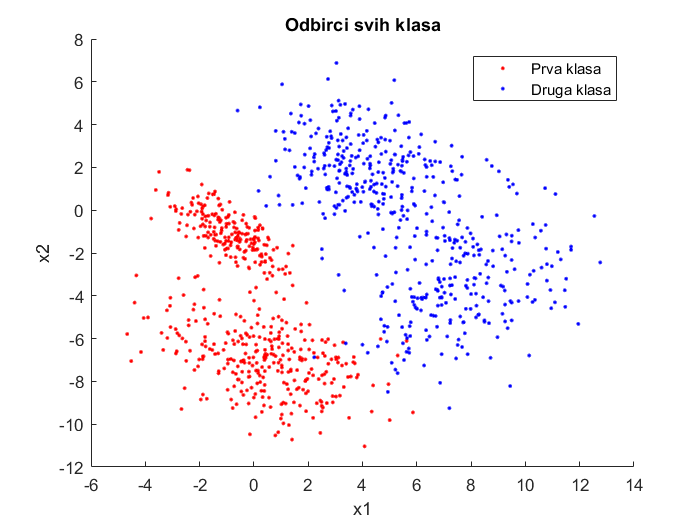
\includegraphics[scale=.5]{pictures/3/LinClass}
\caption{Одбирци}\label{fig:linClass}
\end{figure}
\subsubsection{Пројектовање линеарног класификатора методом ресупституције}
Линеарни класификатор је један од најједноставнијих класификатора, Иако у већини случајева није оптималан јер класе не морају да буду линеарно сепарабилне, често се користи због једноставности. Дискриминациона функција је линеарна и правило одлучивања гласи:
$$h(X) = V^T + v_0 < 0 \implies X \in \omega_1$$
$$h(X) = V^T + v_0 >0 \implies X \in \omega_2$$
Метод који је коришћен је метод ресупституције. Првобитно су процењени вектори средњих вредности $M1Approx, M2Approx$ и коваријационе матрице $S1Approx, S2Approx$, то је коришћено одсечком кода \ref{piece:expVarApprox}.

\begin{lstlisting}[caption={Процена математичког очекивања и ковариационе матрице},label={piece:expVarApprox}]
M1Approx = mean(X1)';
M2Approx = mean(X2)';

S1Approx = cov(X1);
S2Approx = cov(X2); 
\end{lstlisting}
Потом се у сваком кораку мења вредност параметра $s \in \left[ 0, 1\right] $,
и за свако $s$ одреди се вектор :
$$V=\left[ s * S1Approx + (1 - s)*S2Approx\right]^{-1}(M2Approx - M1Approx)$$
Потом се вектор $X$ пројектује на вектор $V$:
$$y_j^{(i)} = V^T X_j^{(i)}, i = 1, 2, j=1, ... N_i$$
где је $N_i$ број облика из $i$-те класе, а $X_j^{(i)}$ $j-$ти обучавајући вектор из $i$-те класе. Затим се $v_0$ мења да се добије најмања грешка. Мења се у опсегу $\left[ -max(max(y_j^{(i)}, max(y_j^{(2)})), -min(min(y_j^{(1)}, min(y_j^{(2)}))\right]$. На крају процедуре бира се оно $s$ за које је број погрешно класификованих објеката (односно грешка) најмањи. 
На слици \ref{fig:sDep} имамо како се $s$ мења у интервалу $\left[0, 1\right]$. Можемо да приметимо да је минимална вредност било која између $0$ и $0, 15$, стога бирамо $0$. 

\begin{figure}[htb!]
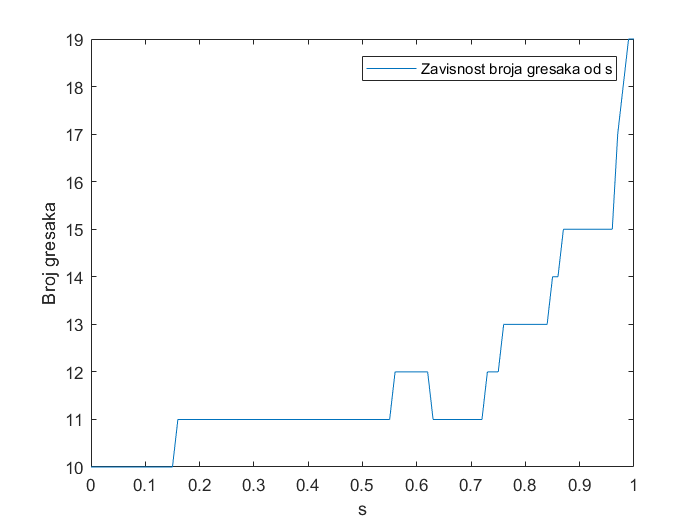
\includegraphics[scale=.6]{pictures/3/sDep}
\centering
\caption{Зависност броја грешака од $s$}\label{fig:sDep}
\end{figure}
За овај случај се добија $V =[1,5254 1.1170]^T, v_0 = -0,6212$ што се види на слици \ref{fig:linClassDisc}. Такође треба приметити да је број грешака 10 што значи да је грешка $1\%$.

\begin{figure}[htb!]
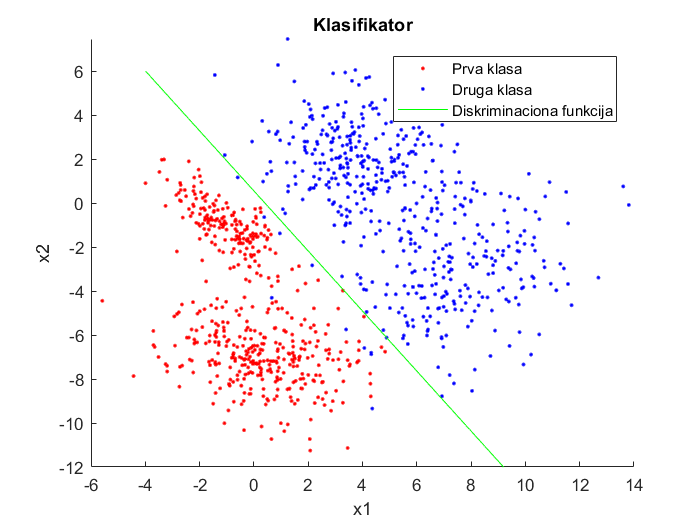
\includegraphics[scale=.6]{pictures/3/LinClassDisc}
\centering
\caption{Одбирци}\label{fig:linClassDisc}
\end{figure}

Код којим је одрађено претходно је одсечак кода \ref{piece:linClassProj}.

\begin{lstlisting}[caption={Пројектовање линеарног класификатора},label={piece:linClassProj}]
step = 0.01;
s = 0 : step : 1;
num_s = length(s);
for i = 1 : num_s
    V = (s(i) * S1Approx  + (1 - s(i)) * S2Approx) \ (M2Approx - M1Approx);
    Y1 = X1 * V;
    Y2 = X2 * V;
    
    downLimit = -max(max(Y1), max(Y2));
    upLimit = -min(min(Y1), min(Y2));
    
    V0 = downLimit : step : upLimit;
    
    minError = size(Y1, 1) + size(Y2, 1);
    minIdx = 0;
    
    V0Num = length(V0);
    
    for j = 1 : V0Num
        v0 = V0(j);
        wrongClass1 = nnz(Y1 > -v0);
        wrongClass2 = nnz(Y2 < -v0);
        wrongClass = wrongClass1 + wrongClass2;
        if (wrongClass < minError)
            minError = wrongClass;
            minIdx = j;
        end
    end
    epsilon(i) = minError;
    V0Min(i) = V0(minIdx);
    
end

[epsilon, idx] = min(epsilon);

sVal = s(idx);

V = (sVal * S1Approx  + (1 - sVal) * S2Approx) \ (M2Approx - M1Approx)
v0 = V0Min(idx)

\end{lstlisting}

\subsubsection{Метод жељеног излаза}
Поновићемо поступак пројектовања линеарног класификатора над датим класама, али овога пута методом жељеног излаза. Код ове методе линија класификациона линија се формаиа тако да за исправно класификован објекат увек буде позитивна:
$$h(X) = -V^T - v_0 > 0 \implies X \in \omega_1$$
$$h(X) = V^T + v_0 > 0 \implies X \in \omega_2$$
Да би се то постигло уводи се нови улазни вектор:
$$Z=[-1 -X_1 .... -X_n]^T,X\in \omega_1$$
$$Z=[1 X_1 .... X_n]^T,X\in \omega_2$$
Проблем се своди на одређивање вектора $W_{(n+1)\times1}$ за који ће што више одбирака $Z$ да испуне релацију $h(Z) = W^TZ > 0$. Критеријумска функција која је најзахвалнија за минимизацију је:
$$\overline{\varepsilon^2} = \frac{1}{N} \sum_{j=1}^N (W^TZ_j - \gamma(Z_j))^2$$
Применом парцијалног извода на њу, и изједначавањем са 0, добија се $U^TW = \Gamma$.
Дата једначина се решава псеудоинверзијом:
$$W = (UU^T)^{-1}U \Gamma,$$
где је $U=[Z_1 Z_2 ... Z_n]$ матрица узорака, а $\Gamma=[\gamma(Z_1) ... \gamma(Z_n)]]^T$ матрица жељених излаза.
Често се за матрицу жељених излаза узима јединични вектор. Одсечак кода \ref{piece:linClassExp} имплементира методу жељеног излаза. 

\begin{lstlisting}[caption={Метода очекиваног излаза},label={piece:linClassExp}]
U = zeros(3, num_points * 2);
G = ones(num_points * 2, 1);
for i = 1 : num_points
    U(:, 2 * i - 1) = [-1 -X1(i, :)];
    U(:, 2 * i) = [1 X2(i, :)];
end

W = U * U' \ U * G;

xIt = -6 : 0.01 : 14;
yIt = -12 : 0.01 : 6;
hExpectedOutput = zeros(length(xIt), length(yIt));
for i = 1 : length(xIt)
    for j = 1 : length(yIt)
        hExpectedOutput(i, j) = [1 xIt(i) yIt(j)] * W;
    end
end
\end{lstlisting}

Добијена функција је $h(X) = -0,2581 + 0,20417_1 + 0,1166x_2$ је приказан на слици \ref{fig:expClassNorm}.
Грешка се рачуна функцијом чији је одсечак кода \ref{piece:linClassExpErr}. 
\begin{figure}[htb!]
\centering
\includegraphics[scale=1]{pictures/3/ExpClassNorm}
\caption{Дискриминациона функција код методе очекиваног излаза}\label{fig:expClassNorm}
\end{figure}

\begin{lstlisting}[caption={Метода очекиваног излаза - грешка},label={piece:linClassExpErr}]
function [epsilon1, epsilon2, epsilon] = errorEstimationEO(U, W, num_points)
    Y = U' * W;
    epsilon = numel(Y(Y < 0)) / (2 * num_points);
    epsilon1 = 0;
    epsilon2 = 0;
    for i = 1 : num_points
        epsilon1 =  (Y(2 * i - 1) < 0) + epsilon1;
        epsilon2 = (Y(2 * i) < 0) + epsilon2;
    end
    epsilon1 = epsilon1 / num_points;
    epsilon2 = epsilon2 / num_points;
end
\end{lstlisting}
Добијене грешке су $\varepsilon_2 = 0,034, \varepsilon_1=0,004, \varepsilon = 0.019$.
Можемо да приметимо да је $\varepsilon_2$ много већа него $\varepsilon_1$. Ако бисмо желели да је смањимо науштрб грешке $\varepsilon_1$ онда бисмо очекиване излазе за елементе који припадају другој класи морали да повећамо. Када то урадимо добија се$\varepsilon_1 = 0.008, \varepsilon=0,024, \varepsilon=0,016$. На слици \ref{fig:expClassNorm} се налази и новодобијена функција. Уопштено ако имамо неку грешку која је већа и желимо да је умањимо методом жељеног излаза, само треба да повећамо жељене излазе за тип грешке који желимо да смањимо.

Ако бисмо желели да минимизујемо свеукупну грешку тад би свим тачкама у близини дискриминационе функције требали да повећамо вредност.  Ако итеративно понављамо дату операцију повећавања добијемо низ дискриминационих функција које конвергирају као на слици \ref{fig:expClassConv} жутој линији. Грешка се смањује и $\varepsilon =0,015$ након ове операције, што је мање него првобитна свеукупна грешка. Одсечак кода \ref{piece:linClassConv} приказује имплементацију претходно наведеног. 
\begin{figure}[htb!]
\centering
\includegraphics[scale=1]{pictures/3/ExpClassConv}
\caption{Низ дискриминационих функција код методе очекиваног излаза}\label{fig:expClassConv}
\end{figure}

\begin{lstlisting}[caption={Метода очекиваног излаза - конвергирање},label={piece:linClassConv}]
U = zeros(3, num_points * 2);
G = ones(num_points * 2, 1);
for i = 1 : num_points
    U(:, 2 * i - 1) = [-1 -X1(i, :)];
    U(:, 2 * i) = [1 X2(i, :)];
end
for t = 1 : 10

    W = U * U' \ U * G;
    xIt = -6 : 0.01 : 14;
    yIt = -12 : 0.01 : 6;
    hExpectedOutput = zeros(length(xIt), length(yIt));
    for i = 1 : length(xIt)
        for j = 1 : length(yIt)
            hExpectedOutput(i, j) = [1 xIt(i) yIt(j)] * W;
        end
    end

    [e1, e2, e] = errorEstimationEO(U, W, num_points);

    fprintf("ExpClose : Greska %.3f Greska1 : %.3f Greska 2 %.3f\n", e, e1, e2);
    if (t == 10)
        contour(xIt,yIt,hExpectedOutput',[0 0],'y');
    else
        contour(xIt,yIt,hExpectedOutput',[0 0],'g');
    end
    Y = U' * W;
    idx = find(Y(1:num_points) < 0.1);
    for i = 1:length(idx)
        G(idx(i)) = 10;
    end
end
\end{lstlisting}

\subsection{Kвадратни класификатор}

Представља сложељнију форму класификатора. Користи се кад две класе нису линеарно сепарабилне. Општа форма квадратног класификатора је:
$$h(X) = X^TQX + V^TX + v_0 < 0 \implies X\in \omega_1$$
$$h(X) = X^TQX + V^TX + v_0 > 0 \implies X\in \omega_2$$
Да би се могао пројектовати неком од постојећих метода, треба да се изврши првидна линеаризација квадратног класификатора. То ћемо учинит на следећи начин:
$$h(X) = q_{11} x_1^2 + q_{22}x_2^2 + q_{12}x_1x_2  + v_1x + v_2x_2 + v_0 = W^TZ > 0 $$
где је улазни вектор 
$$Z=[-1 -x_1 -x_2 -x_1x_2 -x_1^2 -x_2^2]^T, X\in \omega_1$$
$$Z=[1 \, x_1 \, x_2\,  x_1x_2\,  x_1^2\,  x_2^2]^T, X\in \omega_2$$
вектор параметара $W = [v_0 v_1 v_2 q_{12} q_{11} q_{22}$

За почетак генерисаћемо одбирке двеју дводимензионалних класа чије су функције густине вероватноће у облику бимодалних Гаусових расподела:
\\
$$f_1(X) = P_{11} N(M_{11}, \Sigma_{11}) + P_{12} N(M_{12}, \Sigma_{12})$$
$$f_2(X) = P_{21} N(M_{21}, \Sigma_{21}) + P_{22} N(M_{22}, \Sigma_{22}),$$
при чему вероватноће, средње вредности и коваријационе матрице имају следеће вредности:
$$P_{11} = 0,6,  M_{11} = \begin{bmatrix}
   0,5\\
   -7
\end{bmatrix}, 
S_{11} = \begin{bmatrix}
				   3,5 & -1\\
				   -1 & 2,2
				\end{bmatrix},
P_{12} = 0,4,  M_{12} = \begin{bmatrix}
										   12\\
										   6
										\end{bmatrix}, 
S_{12} = \begin{bmatrix}
				   1,3 & -0,9\\
			   	-0,9 &  1.2
				\end{bmatrix}
$$				
$$P_{21} = 0,45,  M_{21} = \begin{bmatrix}
   7,5\\
   -3,5
\end{bmatrix}, 
S_{21} = \begin{bmatrix}
				   4 & 1,1\\
				   1,1 & 4
				\end{bmatrix},
P_{22} = 0,55,  M_{22} = \begin{bmatrix}
										   4\\
										   2
										\end{bmatrix}, 
S_{22} = \begin{bmatrix}
				   3 & -0,8\\
			   	-0,8 &  3
				\end{bmatrix}
$$
Применом методе псудоинверзије добијамо да ус вектор параметара и дискриминациона функција:
$$W = [0,7240,\,0,0622\,\,0,1785\,\, -0,0310\,\, -0,0061\,\, 0,0105]$$
$$h(X) = -0,7240 +0,0622x_1+0,1785x_2 -0,0310x_1x_2 -0,0061x_1^2 +0,0105x_2^2$$
Добијају се грешке $\varepsilon=0,013, \varepsilon_1 = 0,024, \varepsilon_2=0,002$. Дискриминациона функција и одбирци су приказани на слици \ref{fig:quadClass}.

\begin{figure}[htb!]
\centering
\includegraphics[scale=1]{pictures/3/QuadClass}
\caption{Квадратни класификатор}\label{fig:quadClass}
\end{figure}